%%%% NAVIGATIONAL TECHNIQUES %%%%
\chapter{Review of existing navigational methods}\label{chap:03_Navigation_Techniques}
As mentioned in \secref{sec:01_Introduction:Background}, the goal of virtual navigation is to reconstruct, at a specified position (e.g., the location of a listener), a sound field that has been measured from one or more known locations (e.g., the locations of ambisonics microphones).
In this section, we review existing methods for such virtual navigation of ambisonics-encoded sound fields.
The methods reviewed here are listed in \tabref{tab:01_Introduction:Methods} (although not all those methods listed in the table are reviewed here).
We first present a general mathematical formulation of the navigation problem in \secref{sec:03_Navigation_Techniques:Problem_Formulation} in order to establish a consistent framework and nomenclature for describing the methods.
We then describe several existing navigational methods: in \secref{sec:03_Navigation_Techniques:Extrapolation_Methods}, we present three linear extrapolation-based navigational methods and, in \secref{sec:03_Navigation_Techniques:Interpolation_Methods}, we present three (two linear and one parametric) interpolation-based navigational methods.
The performance of several of these methods will be characterized in \chaprefthru{chap:07_Characterization_Extrapolation}{chap:09_Thiergart_Comparison}.
%Several of these methods have also been implemented in a MATLAB toolkit, which is freely available online.\citefooturl{AmbiNavToolkitURL}

\section{Mathematical formulation}\label{sec:03_Navigation_Techniques:Problem_Formulation}
Generally, we seek the ambisonics signals, $a_n$, up to order $L_\text{out}$, that describe the sound field in the vicinity of the listener, located at $\vec{r}_0$.
Using \eqnref{eq:02_Acoustical_Theory:Finite_Order_Expansion}, this potential field is given by
\begin{equation}\label{eq:03_Navigation_Techniques:Output_Potential_Field}
\psi(k,\vec{r} + \vec{r}_0) = \sum_{n=0}^{N_\text{out} - 1} 4\pi (-i)^l A_n(k) j_l(kr) \frac{Y_n(\hat{r})}{\|Y_n\|^2} ,
\end{equation}
where $N_\text{out} = (L_\text{out} + 1)^2$ and $A_n = \mathcal{F} \left[ a_n \right]$.

We take as inputs to each navigational method a set of measured (or synthesized) ambisonics signals, $b_n$, up to order $L_\text{in}$, that describe the sound field in the vicinity of the microphone (either real or virtual), which is located at $\vec{u}$.
Again using \eqnref{eq:02_Acoustical_Theory:Finite_Order_Expansion}, this potential field is given by
\begin{equation}\label{eq:03_Navigation_Techniques:Input_Potential_Field}
\psi(k,\vec{r} + \vec{u}) = \sum_{n=0}^{N_\text{in} - 1} 4\pi (-i)^l B_n(k) j_l(kr) \frac{Y_n(\hat{r})}{\|Y_n\|^2} ,
\end{equation}
where $N_\text{in} = (L_\text{in} + 1)^2$ and $B_n = \mathcal{F} \left[ b_n \right]$.
Thus, estimation of $a_n$ from $b_n$ amounts to a translation from the position of the microphone, $\vec{u}$, along the vector $\vec{r}_0 - \vec{u}$, as illustrated in \figref{fig:03_Navigation_Techniques:Problem_Formulation}.

% Diagram of source/mic positions
\begin{figure}[t]
\centering
  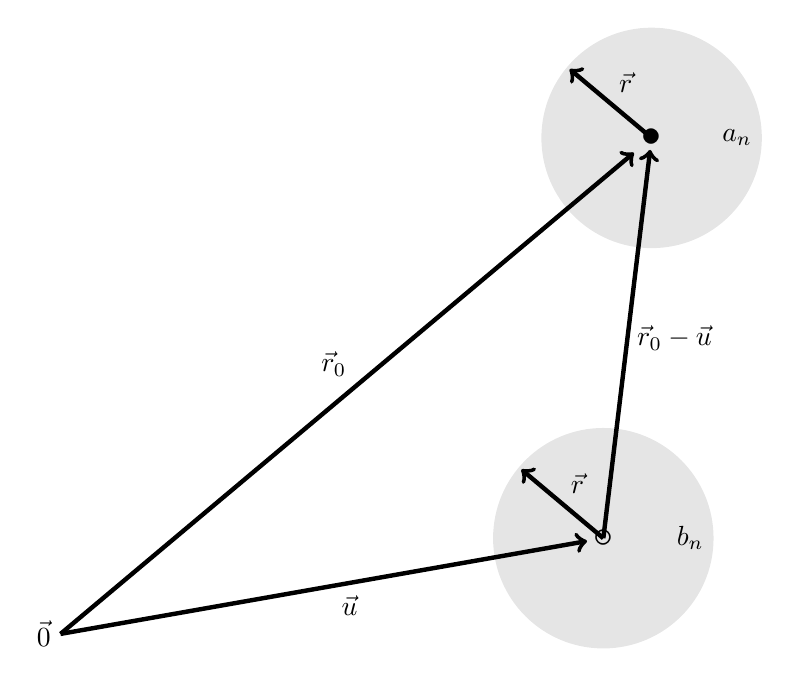
\begin{tikzpicture}[scale=5]
% Parameters
\def\lengthscale{1.4};
\def\radius{0.2*\lengthscale}
\def\arrowStart{0};
\def\arrowScale{0.97};

\pgfmathsetmacro\evalX{cos(140)*\radius}
\pgfmathsetmacro\evalY{sin(140)*\radius}

\pgfmathsetmacro\micX{cos(10)*\lengthscale}
\pgfmathsetmacro\micY{sin(10)*\lengthscale}

\pgfmathsetmacro\listenerX{cos(40)*1.4*\lengthscale}
\pgfmathsetmacro\listenerY{sin(40)*1.4*\lengthscale}

% Arrows
%\draw[ultra thick,->] ({\arrowStart*\evalX},{\arrowStart*\evalY}) -- (\arrowScale*\evalX,\arrowScale*\evalY);
%\node[above right] at (0.5*\evalX,0.5*\evalY){$\vec{r}$};
%\fill [color=black,opacity=0.1] (0,0) circle (\radius);

\draw[ultra thick,->] ({\arrowStart*\evalX+\micX},{\arrowStart*\evalY+\micY}) -- (\arrowScale*\evalX+\micX,\arrowScale*\evalY+\micY);
\node[above right] at (0.5*\evalX+\micX,0.5*\evalY+\micY){$\vec{r}$};
\fill [color=black,opacity=0.1] (\micX,\micY) circle (\radius);

\draw[ultra thick,->] ({\arrowStart*\evalX+\listenerX},{\arrowStart*\evalY+\listenerY}) -- (\arrowScale*\evalX+\listenerX,\arrowScale*\evalY+\listenerY);
\node[above right] at (0.5*\evalX+\listenerX,0.5*\evalY+\listenerY){$\vec{r}$};
\fill [color=black,opacity=0.1] (\listenerX,\listenerY) circle (\radius);

\draw[ultra thick,->] ({\arrowStart*\micX},{\arrowStart*\micY}) -- (\arrowScale*\micX,\arrowScale*\micY);
\node[below right] at (0.5*\micX,0.5*\micY){$\vec{u}$};

\draw[ultra thick,->] ({\arrowStart*\listenerX},{\arrowStart*\listenerY}) -- (\arrowScale*\listenerX,\arrowScale*\listenerY);
\node[above left] at (0.5*\listenerX,0.5*\listenerY){$\vec{r}_0$};

\draw[ultra thick,->] ({(\listenerX-\micX)*\arrowStart+\micX},{(\listenerY-\micY)*\arrowStart+\micY}) -- ({(\listenerX-\micX)*\arrowScale+\micX},{(\listenerY-\micY)*\arrowScale+\micY});
\node[right] at ({(\listenerX-\micX)*0.5+\micX},{(\listenerY-\micY)*0.5+\micY}){$\vec{r}_0 - \vec{u}$};

% Origin
\node[left] at (0,0){$\vec{0}$};

% Mic position
\node at (\micX,\micY){\Large $\circ$};
\node[left] at (\micX+\radius,\micY){$b_n$};

% Listener position
\node at (\listenerX,\listenerY){\Large $\bullet$};
\node[left] at (\listenerX+\radius,\listenerY){$a_n$};
\end{tikzpicture}
  \caption[Diagram of microphone and listener positions.]{
  Diagram of microphone and listener positions.
  The empty circle indicates the microphone position,
  the filled circle indicates the listener position, and
  the shaded disks indicate the regions of the sound field represented by the corresponding ambisonics expansions.}
  \label{fig:03_Navigation_Techniques:Problem_Formulation}
\end{figure}

In general, we will consider arrays of $P$ ambisonics microphones, where the $p^\text{th}$ microphone is located at $\vec{u}_p$ for $p \in [1,P]$.
For microphones of order $L_\text{in}$,\footnote{The order of the ambisonics microphone is generally determined by the number of capsules in the assembly.} each microphone captures $N_\text{in} = (L_\text{in} + 1)^2$ ambisonics signals, which we represent with a vector, $\mathbf{b}_p$.
(See \chapref{chap:02_Acoustical_Theory} for a review of ambisonics conventions and theory.)
%In general, ambisonics navigation techniques aim to approximate, up to order $L_\text{out}$ and with $N_\text{out} = (L_\text{out} + 1)^2$ terms, the exact ambisonics signals, $\mathbf{a}$, of the sound field at a listening position $\vec{r}_0$.
In the case of extrapolation methods, for which $P = 1$, we omit the subscripts for $\vec{u}_1$ and $\mathbf{b}_1$ (and instead simply use $\vec{u}$ and $\mathbf{b}$, respectively).

% include operator notation, tikz block diagram

\section{Extrapolation methods}\label{sec:03_Navigation_Techniques:Extrapolation_Methods}
In this section, we review three linear extrapolation-based navigational methods:
\begin{enumerate}
\item virtual ambisonics \citep[section 3.1]{TylkaChoueiri2015},
\item plane-wave translation \citep{SchultzSpors2013}, and
\item ambisonics translation \citep{GumerovDuraiswami2005,MenziesAlAkaidi2007a,Zotter2009PhD}.
\end{enumerate}

%% VIRTUAL AMBISONICS %%
\subsection{Virtual ambisonics}\label{sec:03_Navigation_Techniques:VA_Technique}
The first navigational method we consider involves simulating ambisonics playback over a virtual array of loudspeakers (hereafter called ``virtual ambisonics'').
In this case, virtual navigation requires only that each loudspeaker signal be appropriately attenuated and delayed based on the distance of the listener to that loudspeaker.
The process of decoding ambisonics signals of order $L_\text{in}$ to $Q$ loudspeakers is reviewed in \secref{sec:02_Acoustical_Theory:VA_Binaural}, which converts the $N_\text{in}$ recorded ambisonics signals, $b_n$, into a set of loudspeaker signals, $g_q$.

Here we model the virtual loudspeakers as point-sources,\footnote{Note that we could have instead modeled the loudspeakers as plane-wave sources, infinitely far away from the listener. However, we chose to use finite-distance virtual loudspeakers so that this technique will differ more significantly from the plane-wave expansion technique described in \secref{sec:03_Navigation_Techniques:PW_Technique}.} where the $q^\text{th}$ loudspeaker is placed at $\vec{v}_q$ and is driven with a (Fourier-transformed) signal $G_q = \mathcal{F} \left[ g_q \right]$.
%Each loudspeaker then produces a potential field given by
%\begin{equation}\label{eq:03_Navigation_Techniques:Point_Source}
%\psi_q(k,\vec{r}) = \frac{e^{i k \left\| \vec{r} - \vec{v}_q \right\|}}{\left\| \vec{r} - \vec{v}_q \right\|} G_q(k),
%\end{equation}
%where we have used \eqnref{eq:02_Acoustical_Theory:PointSource}.
%The total potential field produced by virtual ambisonics playback is then given by
%\begin{equation}\label{eq:03_Navigation_Techniques:VA_Rendered_Field}
%\psi(k,\vec{r}) = \sum_{q = 1}^Q \frac{e^{i k \left\| \vec{r} - \vec{v}_q \right\|}}{\left\| \vec{r} - \vec{v}_q \right\|} G_q(k).
%\end{equation}
These signals are then re-encoded into ambisonics up to an arbitrary order, $L_\text{out}$, at the position of the listener, $\vec{r}_0$, via \eqnref{eq:02_Acoustical_Theory:PointSource_An}, such that
\begin{equation}\label{eq:03_Navigation_Techniques:VA_Output}
A_n(k) = \sum_{q = 1}^Q i^{l+1} k h_l(k \left\| \vec{v}_q - \vec{r}_0 \right\|) Y_n \left( \frac{\vec{v}_q - \vec{r}_0}{\left\| \vec{v}_q - \vec{r}_0 \right\|} \right) G_q(k).
\end{equation}

Note that, for binaural playback, we can skip the step of re-encoding to ambisonics and instead simply filter the point-source signals (appropriately attenuated and delayed based on distance to the listener) by the corresponding HRTFs of the listener.
However, for mathematical consistency when comparing different navigational methods, we choose an ambisonics output.

%To binaurally render the sound field described by~\eqnref{eq:03_Navigation_Techniques:VA_Rendered_Field} for a listener at position $\vec{r}_0$, the left and right binaural potentials (indicated by the superscripts ``$\text{L}$'' and ``$\text{R}$,'' respectively) are computed by
%\begin{equation}\label{eq:VA_Binaural}
%\psi_\text{VA}^\text{L,R}(k,\vec{r}_0) = \sum_{q=1}^{Q} \frac{e^{i k \left\| \vec{v}_q - \vec{r}_0 \right\|}}{\left\| \vec{v}_q - \vec{r}_0 \right\|} G_q(k) \cdot H^\text{L,R} \left( k, \frac{\vec{v}_q - \vec{r}_0}{\left\| \vec{v}_q - \vec{r}_0 \right\|} \right),
%\end{equation}
%where $H^\text{L,R}(k,\hat{v})$ is the far-field HRTF for a source in the direction $\hat{v}$.

%% PLANE-WAVE TRANSLATION %%
\subsection{Plane-wave translation}\label{sec:03_Navigation_Techniques:PW_Technique}
The second navigational method we consider uses a plane-wave decomposition of the finite-order potential field.
This technique was developed by \citet{SchultzSpors2013}, who showed that translation can be achieved by applying a frequency-domain phase-factor (or group delay in the time domain) to each plane-wave term, based on the direction of travel of the listener relative to the propagation direction of each plane-wave.

Beginning with \eqnref{eq:02_Acoustical_Theory:PW_Quadrature_Rendered_Field}, we see that, for each term in this summation, the potential field at $\vec{r} + \vec{r}_0$ differs only by a phase-factor: $e^{-i k \hat{v}_q \cdot \vec{r}_0}$.
We combine this factor into the signature function to define the \textit{translated signature function}, $\mu'$, given by \citep{MenziesAlAkaidi2007b}
\begin{equation}\label{eq:03_Navigation_Techniques:PW_Translation}
\mu'(k,\hat{v}_q;\vec{r}_0) = \mu(k,\hat{v}_q) e^{-i k \hat{v}_q \cdot \vec{r}_0},
\end{equation}
where the dot product in the exponential indicates that the $q^\text{th}$ plane-wave term undergoes a time delay proportional to the distance traveled parallel to the propagation direction, $-\hat{v}_q$, of that term.
Effectively, this operation translates the expansion center from the origin to $\vec{r}_0$.

Given a set of measured ambisonics signals, $\mathbf{b}$, up to order $L_\text{in}$, we can substitute $B_n$ for $A_n$ in \eqnref{eq:02_Acoustical_Theory:A2mu} to compute the measured signature function, $\mu$.
Then, using \eqnref{eq:03_Navigation_Techniques:PW_Translation},
we compute the translated signature function, $\mu'(k,\hat{v}_q;\vec{r}_0 - \vec{u})$,
where $\vec{u}$ is the position of the ambisonics microphone and $\vec{r}_0$ is the position of the listener.
By substituting $\mu'$ for $\mu$ in~\eqnref{eq:02_Acoustical_Theory:mu2A_Quadrature}, we then convert this translated signature function back into ambisonics signals, up to an arbitrary order, $L_\text{out}$, yielding ambisonics signals for the listener, $\mathbf{a}$.

Note that, as with the virtual ambisonics method, one could render the translated plane-wave terms directly to binaural by filtering each signal by the appropriate HRTF.
Here, however, we choose to generate an ambisonics output for mathematical consistency across different navigational methods.

%% AMBISONICS TRANSLATION %%
\subsection{Ambisonics translation}\label{sec:03_Navigation_Techniques:SR_Technique}
The third navigational method we consider was first described by \citet{MenziesAlAkaidi2007a}, and entails computing a new set of ambisonics signals by re-expanding the sound field about a translated expansion center using frequency-domain translation coefficients.

Following the theory described in \secref{sec:02_Acoustical_Theory:Ambisonics_Translation}, the ambisonics signals for the listener, $\mathbf{a}(k)$, are given by
\begin{equation}\label{eq:03_Navigation_Techniques:Forward_Ambisonics_Translation}
\mathbf{a}(k) = \left( \mathbf{T}(k, \vec{r}_0 - \vec{u}) \right)^\text{T} \cdot \mathbf{b}(k),
\end{equation}
where again $\vec{u}$ is the position of the ambisonics microphone (i.e., the expansion center for $\mathbf{b}$) and $\vec{r}_0$ is the position of the listener (cf.~\eqnref{eq:02_Acoustical_Theory:Translated_Expansion_Coefficients_Matrix}).
Recall that the translated expansion coefficients $A_n$ can be computed to an arbitrary order $L_\text{out}$.

The potential field at $\vec{r} + \vec{r}_0$ obtained through translation along $\vec{r}_0 - \vec{u}$ is then given by \eqnref{eq:03_Navigation_Techniques:Output_Potential_Field}.
It is important to note that the re-expanded field is still limited in accuracy and region of validity by the original expansion.
In other words, with increasing $L_\text{out}$, the re-expanded field approaches the original \textit{order-limited} field, not the incident field.

According to the inequality given in \eqnref{eq:01_Introduction:kr_Inequality}, the accuracy of the translated ambisonics signals will degrade with increasing frequency and distance away from the microphone.
To explore this behavior in the frequency domain, we compute the frequency response induced by translation away from the microphone and plot, in \figref{fig:03_Navigation_Techniques:SRE_RollOff}, the magnitude responses corresponding to various translation distances and input orders.%
\footnote{Simulations of this type are described in more detail in \chapref{chap:06_Simulation_Framework}.
Briefly, in this case, the sound field consists of a single point-source placed at $\vec{s}_0 = (2.5, 0, 0)$~m, a microphone of order $L_\text{in} \in [1,5]$ placed at $\vec{u} = (0.25, 0, 0)$~m, and a variable listener position of $\vec{r}_0 = (x_0, 0, 0)$ with $x_0 \in [0, 0.25]$~m.
A diagram of this geometry is shown in \figref{fig:06_Simulation_Framework:Point_Geometry}.
The microphone signals are given by \eqnref{eq:02_Acoustical_Theory:PointSource_An} and we have omitted the near-field compensation high-pass filter defined in \eqnref{eq:02_Acoustical_Theory:NearField_HPF}.
The effective frequency response induced by translating from $\vec{u}$ to $\vec{r}_0$ via \eqnref{eq:03_Navigation_Techniques:Forward_Ambisonics_Translation} is then given by the ratio of the translated zeroth-order ambisonics signal, $A_0(k)$, to the zeroth-order reference ambisonics signal, $B_0(k)$, that would have been measured at $\vec{r}_0$.}
From these plots, we see that translation effectively acts as a low-pass filter, the corner frequency of which approximately corresponds to $k \propto L_\text{in} / \| \vec{r}_0 - \vec{u} \|$.
(Although not shown here, it can be verified that this behavior also holds across all source and listener positions.
See, for example, \figref{fig:07_Characterization_Extrapolation:Azimuth_Dependence:SRE}, which shows this behavior over multiple source azimuths.)

\begin{figure}[t]
  \centering
  \begin{subfigure}[b]{0.49\textwidth}
    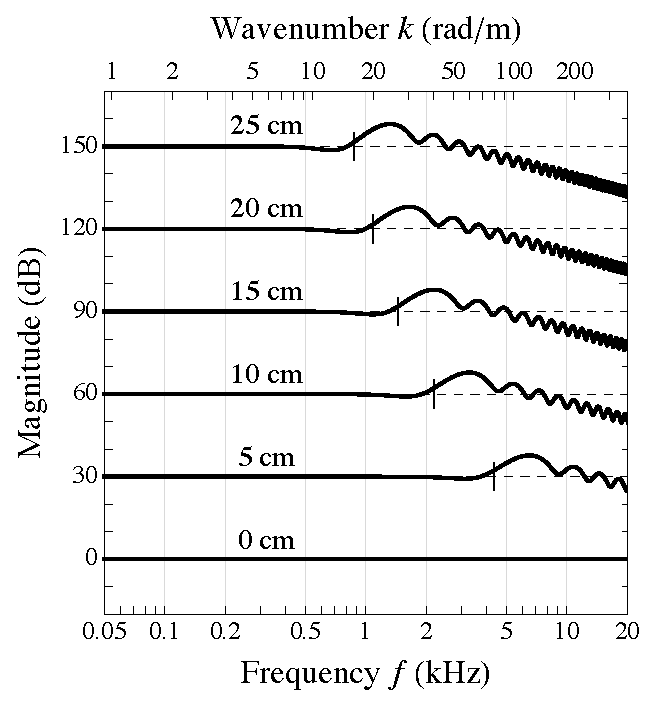
\includegraphics[width=\textwidth]{03_navigational_techniques/figures/freqResp_listenerPos_sre.eps}
    \caption{Varying $\| \vec{r}_0 - \vec{u} \|$; fixed $L_\text{in} = 4$}
    \label{fig:03_Navigation_Techniques:SRE_RollOff:ListenerPos}
  \end{subfigure}
  \hfill
  \begin{subfigure}[b]{0.49\textwidth}
    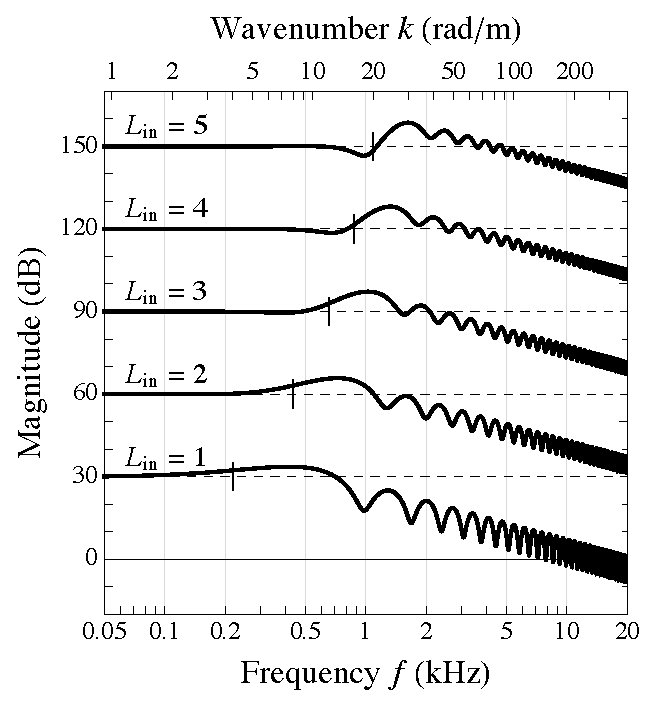
\includegraphics[width=\textwidth]{03_navigational_techniques/figures/freqResp_inputOrders_sre.eps}
    \caption{Varying $L_\text{in}$; fixed $\| \vec{r}_0 - \vec{u} \| = 0.25$~m}
    \label{fig:03_Navigation_Techniques:SRE_RollOff:InputOrders}
  \end{subfigure}
  \caption[Magnitude responses caused by the ambisonics translation method.]{
  Magnitude responses caused by the ambisonics translation method for various translation distances (left panel) and input orders (right).
  The bottom axes show frequency in kHz while the top axes show the angular wavenumber $k$.
  The short vertical lines indicate the nondimensional frequency $k \| \vec{r}_0 - \vec{u} \| = L_\text{in}$.
  For legibility, each frequency response is offset by $30$~dB.}
  \label{fig:03_Navigation_Techniques:SRE_RollOff}
\end{figure} %%NOTE%% vertical axis label is too complicated: |A0 / B0ref| or something

To better show the similarities across these different parameters, we plot, in \figref{fig:03_Navigation_Techniques:Nondim_SRE_RollOff}, the same magnitude responses as in \figref{fig:03_Navigation_Techniques:SRE_RollOff}, but now against a normalized wavenumber, $k \| \vec{r}_0 - \vec{u} \| / L_\text{in}$.
As expected, the corner of each effective low-pass filter is located at $k \| \vec{r}_0 - \vec{u} \| / L_\text{in} \approx 1$.
From these plots, we clearly see that the basic shape of the magnitude response is virtually identical across different translation distances (see \figref{fig:03_Navigation_Techniques:Nondim_SRE_RollOff:ListenerPos}), whereas varying the input order yields noticeable differences (\figref{fig:03_Navigation_Techniques:Nondim_SRE_RollOff:InputOrders}).
In particular, increasing the input order decreases the amplitude of, and spacing between, the ``ripples'' that modulate the overall low-pass behavior above the corner.

\begin{figure}[t]
  \centering
  \begin{subfigure}[b]{0.49\textwidth}
    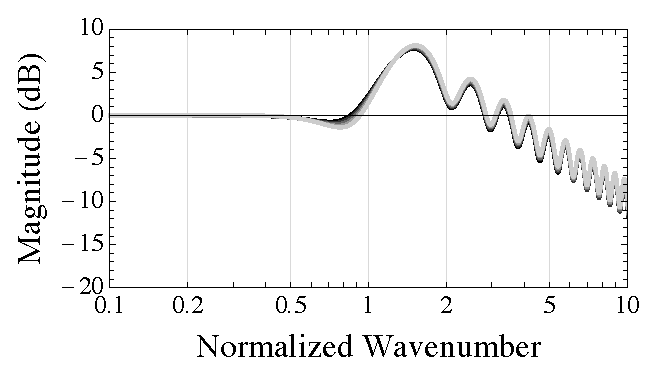
\includegraphics[width=\textwidth]{03_navigational_techniques/figures/nondimFreqResp_listenerPos_sre.eps}
    \caption{Varying $\| \vec{r}_0 - \vec{u} \|$; fixed $L_\text{in} = 4$}
    \label{fig:03_Navigation_Techniques:Nondim_SRE_RollOff:ListenerPos}
  \end{subfigure}
  \hfill
  \begin{subfigure}[b]{0.49\textwidth}
    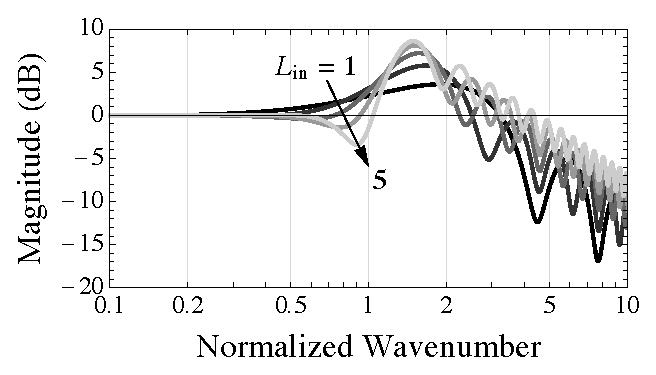
\includegraphics[width=\textwidth]{03_navigational_techniques/figures/nondimFreqResp_inputOrders_sre.eps}
    \caption{Varying $L_\text{in}$; fixed $\| \vec{r}_0 - \vec{u} \| = 0.25$~m}
    \label{fig:03_Navigation_Techniques:Nondim_SRE_RollOff:InputOrders}
  \end{subfigure}
  \caption[Magnitude responses caused by the ambisonics translation method.]{
  Magnitude responses caused by the ambisonics translation method for various translation distances (left panel) and input orders (right), where the lighter gray curves correspond to increasing translation distance or input order, respectively.
  The horizontal axes show the nondimensional wavenumber $k \| \vec{r}_0 - \vec{u} \| / L_\text{in}$.}
  \label{fig:03_Navigation_Techniques:Nondim_SRE_RollOff}
\end{figure}

It is worth noting that translation may also be carried out through the \textit{inverse} (or pseudoinverse if $L_\text{in} \neq L_\text{out}$) operation, such that
\begin{equation}\label{eq:03_Navigation_Techniques:Inverse_Ambisonics_Translation}
\mathbf{a}(k) = \left(\left( \mathbf{T}(k, \vec{u} - \vec{r}_0) \right)^\text{T} \right)^{-1} \cdot \mathbf{b}(k).
\end{equation}
However, as shown in \figref{fig:03_Navigation_Techniques:SRE_RollOff}, the forward translation operation given by~\eqnref{eq:03_Navigation_Techniques:Forward_Ambisonics_Translation} leads to an attenuation (i.e., a ``roll-off'') of high frequencies.
Consequently, the inverse operation will yield excessive high-frequency amplification, unless steps (such as regularization) are taken to mitigate such excessive gains.

In \secref{sec:03_Navigation_Techniques:Pinv_Technique}, a regularized least-squares approach is implemented in an interpolation method that uses multiple ambisonics microphones to estimate the ambisonics signals at the position of the listener.
Consequently, the inverse approach to extrapolation defined in \eqnref{eq:03_Navigation_Techniques:Inverse_Ambisonics_Translation} can be considered a special case of that interpolation method, in which we have only a single array (i.e., $P = 1$) and no regularization is used.

%%%% INTERPOLATION METHODS %%%%
\section{Interpolation methods}\label{sec:03_Navigation_Techniques:Interpolation_Methods}
In this section, we review three interpolation-based navigational methods:
\begin{enumerate}
\item weighted-average interpolation \citep{Southern2009,MarietteKatz2009},
\item regularized least-squares (i.e., pseudoinversion-based) ambisonics interpolation \citep{Samarasinghe2014a,TylkaChoueiri2016}, and
\item time-frequency sound field analysis and modeling \citep{Thiergart2013}.
\end{enumerate}

%%%% Crossfading Method %%%%
\subsection{Weighted-average interpolation}\label{sec:03_Navigation_Techniques:XF_Technique}
In the navigational method proposed by \citet{MarietteKatz2009} and \citet{Southern2009}, a weighted sum of the captured ambisonics signals is computed to obtain an estimate of the ambisonics signals at the listening position, given by
\begin{equation}\label{eq:03_Navigation_Techniques:Crossfading}
\mathbf{\tilde{a}}(k) = \sum_{p=1}^P w_p \mathbf{b}_p(k),
\end{equation}
where the weights are normalized such that
\begin{equation}\label{eq:03_Navigation_Techniques:Weight_Normalization}
\sum_{p=1}^P w_p = 1.
\end{equation}
Note that as the sum in \eqnref{eq:03_Navigation_Techniques:Crossfading} is computed term-by-term, we must have an output order $L_\text{out} \leq L_\text{in}$, where the inequality arises if one chooses to discard higher-order terms captured by the microphones.
Depending on the placement of the microphones in the sound field, the weights $w_p$ may be computed using standard linear or bilinear schemes, for example.

For $P = 2$ microphones, we first define the distance between the two microphones, given by $\Delta = \|\vec{u}_2 - \vec{u}_1\|$.
We then compute the effective position, $y_1$, of the listener, as projected onto the vector connecting the two microphones, such that $y_1$ is given by
\begin{equation}
y_1 = \frac{\langle \vec{r}_0 - \vec{u}_1, \vec{u}_2 - \vec{u}_1 \rangle}{\Delta},
\end{equation}
where $\langle \cdot, \cdot \rangle$ denotes the inner (dot) product of two Cartesian vectors.
From this, linear interpolation weights are given by
\begin{equation}\label{eq:03_Navigation_Techniques:Linear_Interpolation_Weights}
w_1 = 1 - w_2
\quad\quad\text{and}\quad\quad
w_2 = 
\begin{cases}
0 & \text{for}~y_1 \leq 0,\\
y_1/\Delta & \text{for}~0 < y_1 < \Delta,\\
1 & \text{for}~y_1 \geq \Delta.
\end{cases}
\end{equation}

%%%% Pseudoinverse Method %%%%
\subsection{Regularized least-squares ambisonics interpolation}\label{sec:03_Navigation_Techniques:Pinv_Technique}
\citet[section III.A]{Samarasinghe2014a} propose a pseudoinversion-based interpolation method in which they consider the ambisonics signals at the listening position and, using the spherical Fourier-Bessel translation coefficient matrices from \secref{sec:02_Acoustical_Theory:Ambisonics_Translation}, write a system of equations simultaneously describing the ambisonics signals at all $P$ ambisonics microphones.%
\footnote{Note that \citeauthor{Samarasinghe2014a} only carry out their derivation for a two-dimensional sound field, but we have extended it here for three-dimensional sound fields \citep[section 3.2]{TylkaChoueiri2016}.}
That is, for each wavenumber (or frequency) $k$, we can write
\begin{equation}\label{eq:03_Navigation_Techniques:Linear_System}
\mathbf{M}(k) \cdot \mathbf{x}(k) = \mathbf{y}(k),
\end{equation}
where, omitting frequency dependencies,
\begin{equation}\label{eq:03_Navigation_Techniques:Linear_System_Matrices}
\mathbf{M} = 
    \left[ \begin{array}{c}
    \left( \mathbf{T}(-\vec{r}_1) \right)^\text{T} \\
    \left( \mathbf{T}(-\vec{r}_2) \right)^\text{T} \\
    \vdots\\
    \left( \mathbf{T}(-\vec{r}_P) \right)^\text{T}
    \end{array} \right]
,\quad
\mathbf{y} = 
    \left[ \begin{array}{c}
    \mathbf{b}_1\\
    \mathbf{b}_2\\
    \vdots\\
    \mathbf{b}_P
    \end{array} \right],
\end{equation}
and $\vec{r}_p$ is the vector from the $p^\textrm{th}$ microphone to the listening position, given by $\vec{r}_p = \vec{r}_0 - \vec{u}_p$.
Ideally, as $L_\textrm{in} \to \infty$, we should find $\mathbf{x} \to \mathbf{a}$ (the exact ambisonics signals of the sound field at $\vec{r}_0$).
In practice, each microphone captures only $N_\textrm{in}$ ambisonics signals, so each $\mathbf{b}_p$ is a column-vector of length $N_\textrm{in}$ and $\mathbf{y}$ is a column-vector of length $P \cdot N_\textrm{in}$.

In order to ensure that the system in \eqnref{eq:03_Navigation_Techniques:Linear_System} is not under-determined, we define the maximum order for $\mathbf{x}$, given by
\begin{equation}\label{eq:03_Navigation_Techniques:Pinv_Interpolation_Lmax}
L_\textrm{max} = \left\lfloor \sqrt{P \cdot N_\textrm{in}} \right\rfloor - 1,
\end{equation}
where $\lfloor \cdot \rfloor$ denotes rounding down to the nearest integer.
Therefore, $\mathbf{x}$ is a column-vector of length $N_\textrm{max} = (L_\textrm{max} + 1)^2$ and each matrix $\mathbf{T}$ in \eqnref{eq:03_Navigation_Techniques:Linear_System_Matrices} will have dimensions $N_\textrm{max} \times N_\textrm{in}$ (rows $\times$ columns).
Note that by this definition, we will always have $L_\textrm{max} \geq L_\textrm{in}$ irrespective of the number of microphones.

Next, we compute the pseudoinverse (or inverse if $\mathbf{M}$ is square) of $\mathbf{M}$ by first finding its singular value decomposition, given by $\mathbf{M} = \mathbf{U} \Sigma \mathbf{V}^*$, where $(\cdot)^*$ represents conjugate-transposition.
In their original paper, \citet{Samarasinghe2014a} suggest taking a truncated singular value regularization approach such that, for some tolerance level $\sigma_\text{min}$, all singular values $\sigma_n < \sigma_\text{min}$ are set to zero.
This allows us to compute the regularized pseudoinverse of $\mathbf{M}$, given by \citep[Eq.~(17)]{Samarasinghe2014a}
\begin{equation}
\mathbf{L} = \mathbf{M}^{+} = \mathbf{V} \Sigma^{+} \mathbf{U}^*,
\end{equation}
where $(\cdot)^+$ represents pseudoinversion.
Finally, we obtain an estimate of $\mathbf{a}$, given by
\begin{equation}
\mathbf{\tilde{a}}(k) = \mathbf{L}(k) \cdot \mathbf{y}(k).
\end{equation}
Note that, as with the weighted average method, we may choose to drop the higher-order terms in $\mathbf{\tilde{a}}$ such that we keep only up to order $L_\textrm{out}$, where $L_\textrm{out} \leq L_\textrm{max}$.

%%%% Thiergart Method %%%%
\subsection{Sound field analysis and modeling}\label{sec:03_Navigation_Techniques:Thiergart_Method}
In the interpolation method proposed by \citet{Thiergart2013}, the sound field is first analyzed in the time-frequency domain and subsequently modeled as a finite set of monochromatic omnidirectional point sources.
As will become clear below, this method can only use the first-order ambisonics signals, so we must have $L_\text{in} = 1$.
The output signals, however, can be computed to an arbitrary order $L_\text{out}$.
Here, we describe our implementation of this method.

\subsubsection{Sound field analysis}
First, we compute three basic quantities: pressure, acoustic intensity, and diffuseness.
For each microphone, we compute the STFT of each of the first four ambisonics signals, which gives $B^{[p]}_n(\xi,\kappa)$ for $n \in [0,3]$ and where $\xi$ is the index of the time frame, $\kappa$ is the frequency index, and the superscript ``$[p]$'' denotes the microphone index.
Typically, we take an overlap fraction of $R = 0.5$, and set the FFT length to be
\begin{equation}
N_\textrm{FFT} = 2^{\left\lceil \log_2 \left( \frac{F_s}{1-R} \frac{\Delta}{c} \right) \right\rceil},
\end{equation}
where $\lceil \cdot \rceil$ denotes rounding up to the nearest integer, $F_s$ is the sampling rate of the system, and $\Delta$ is again the distance between microphones.
We let the window length also equal $N_\textrm{FFT}$ and choose a Hamming window, as defined in the MATLAB \texttt{hamming} function.\citefooturl{MATLABhammingURL}

Using these signals in the time-frequency domain, we compute the acoustic potential (pressure), given by
\begin{equation}\label{eq:03_Navigation_Techniques:Time-Frequency_Potential}
\psi^{[p]}(\xi,\kappa) = B^{[p]}_0(\xi,\kappa) \sqrt{\frac{4\pi}{\|Y_0\|^2}}.
\end{equation}
We then compute the acoustic intensity vector, $\vec{\nu}^{[p]}_\textrm{I}(\xi,\kappa)$, and the diffuseness parameter, $\Psi^{[p]}(\xi,\kappa)$, as given below in \eqnreftwo{eq:04_Auditory_Models:Intensity_Vector}{eq:04_Auditory_Models:Diffuseness}, respectively.

Using the acoustic intensity vectors, we then triangulate a single source for each time-frequency bin.
For two microphones and with sources restricted to the horizontal plane, this is computed as follows:
\begin{equation}\label{eq:03_Navigation_Techniques:Time-Frequency_Source_Position}
\begin{gathered}
\vec{s}_0(\xi,\kappa) = \vec{u}_1 + c_1 \hat{\nu}^{[1]}_\textrm{I}(\xi,\kappa) = \vec{u}_2 + c_2 \hat{\nu}^{[2]}_\textrm{I}(\xi,\kappa),\\
\implies \vec{u}_2 - \vec{u}_1 = c_1 \hat{\nu}^{[1]}_\textrm{I}(\xi,\kappa) - c_2 \hat{\nu}^{[2]}_\textrm{I}(\xi,\kappa),
\end{gathered}
\end{equation}
where $\vec{s}_0$ is the triangulated source position and $c_1$ and $c_2$ are scalars found for each time-frequency bin.
These scalars are computed by
\begin{equation}\label{eq:03_Navigation_Techniques:Source_Triangulation}
\left[
\begin{array}{c}
c_1 \\
c_2
\end{array}
\right]
 = 
\left[
\begin{array}{cc}
\cos \phi_\textrm{I}^{[1]} & -\cos \phi_\textrm{I}^{[2]} \\[6pt]
\sin \phi_\textrm{I}^{[1]} & -\sin \phi_\textrm{I}^{[2]}
\end{array}
\right]^{-1}
 \cdot 
\left[
\begin{array}{c}
x_2 - x_1 \\
y_2 - y_1
\end{array}
\right],
\end{equation}
where $\phi_\textrm{I}^{[p]}$ denotes the azimuth of $\vec{\nu}_\textrm{I}^{[p]}$ and $x_p$ and $y_p$ denote the $x$ and $y$ components of $\vec{u}_p$, respectively.
Note that the matrix inversion in \eqnref{eq:03_Navigation_Techniques:Source_Triangulation} fails when $\phi_\textrm{I}^{[1]} = \phi_\textrm{I}^{[2]}$, i.e., when the intensity vectors are parallel.
A more general approach for source triangulation, either in three dimensions or for $P > 2$ microphones (or both), is described by \citet[section IV.A]{Thiergart2013}.

\subsubsection{Sound field modeling and synthesis}
The estimated ambisonics output signals are assembled in the time-frequency domain as follows.
For a given listener position $\vec{r}_0$, we let $\vec{s}_0{}' = \vec{s}_0 - \vec{r}_0$ be the position of the triangulated source relative to the listener at each time-frequency bin.
Additionally, we choose a reference microphone with index $p = p_\textrm{ref}$, such that the position of the triangulated source relative to the reference microphone is given by $\vec{s}_{p_\textrm{ref}} = \vec{s}_0 - \vec{u}_{p_\textrm{ref}}$.
By default, we choose as the reference the nearest microphone to the listener.
We further define a direct-to-diffuse ratio parameter, given by
\begin{equation}\label{eq:03_Navigation_Techniques:Direct-to-Diffuse_Ratio}
\Gamma(\xi,\kappa) = \frac{1}{\Psi^{[p_\textrm{ref}]}(\xi,\kappa)} - 1,
\end{equation}
as well as direct and diffuse components of the sound field, respectively, given by
\begin{align}
S_\textrm{dir}(\xi,\kappa) &= \sqrt{\frac{\Gamma(\xi,\kappa)}{1 + \Gamma(\xi,\kappa)}} \frac{\psi^{[p_\textrm{ref}]}}{i k h_0(k s_{p_\textrm{ref}})}, \\
S_\textrm{diff}(\xi,\kappa) &= \sqrt{\frac{1}{1 + \Gamma(\xi,\kappa)}} \psi^{[p_\textrm{ref}]}.
\end{align}
Recall that direct point-source components are encoded into ambisonics using \eqnref{eq:02_Acoustical_Theory:PointSource_An}.
Correspondingly, diffuse sound components are encoded into ambisonics by integrating the ``directivity'' of each ambisonics channel.
That is, the effective ambisonic encoding filters for diffuse sound are given by
\begin{equation}
A_n = \sqrt{\frac{\|Y_n\|^2}{4\pi}}.
\end{equation}
From this, we compute the ambisonics output signals up to order $L_\text{out}$ by
\begin{equation}\label{eq:03_Navigation_Techniques:Thiergart_Synthesis}
\tilde{A}_n(\xi,\kappa) = i^{l+1} k h_l(k s_0{}') Y_n(\hat{s}_0{}') S_\textrm{dir}(\xi,\kappa) + \sqrt{\frac{\|Y_n\|^2}{4\pi}} S_\textrm{diff}(\xi,\kappa),
\end{equation}
which is converted into the time domain via an inverse STFT for all $n \in [0, N_\text{out}-1]$.

\section{Summary of methods}
In this section, we summarize the main equations for, and important differences between, the methods reviewed in this chapter.

\subsection{Extrapolation methods}
The virtual ambisonics and plane-wave translation methods are generally very similar:
both methods entail representing the sound field with a finite number of discrete sources, which are often distributed spherically around the recording point.
They differ, however, in that the virtual ambisonics method represents the sound field using point-sources, whereas the plane-wave translation method uses plane-wave sources.
Consequently, while translation for the plane-wave translation method requires only a simple time-delay term (see \eqnref{eq:03_Navigation_Techniques:PW_Translation}), translation for the virtual ambisonics method additionally requires directional changes and amplification (or attenuation) based on distance changes for each point-source (see \eqnref{eq:03_Navigation_Techniques:VA_Output}).
Nevertheless, due to the similarities between these two methods, in \chapref{chap:07_Characterization_Extrapolation} we omit the virtual ambisonics method and instead focus our analysis only on the plane-wave and ambisonics translation methods.

The ambisonics translation method is categorically different from the other two methods, as it does not seek an alternative representation of the sound field.
Instead, the method operates directly on the ambisonics signals by applying a matrix of frequency-dependent translation coefficients (see \eqnref{eq:03_Navigation_Techniques:Forward_Ambisonics_Translation}).
As demonstrated in \secref{sec:03_Navigation_Techniques:SR_Technique}, these coefficients necessarily introduce a low-pass-like roll-off of high-frequency energy (see \figref{fig:03_Navigation_Techniques:SRE_RollOff}).
The main equations describing these methods are reproduced (in slightly modified forms) in \tabref{tab:03_Navigational_Techniques:Extrapolation_Equations}.

\begin{sidewaystable}
\centering
\begin{tabular}{c|c|c|c}
\textbf{Method} & \textbf{Input Conversion} & \textbf{Translation Operation} & \textbf{Output Conversion} \\\hline\hline
\rule[-1.5cm]{0pt}{3.1cm} Virtual ambisonics & $\begin{bmatrix}
G_{1}(k) \\ G_{2}(k) \\ \vdots \\ G_{Q}(k)
\end{bmatrix} = \mathbf{Y}^{+} \cdot \mathbf{b}(k)$ & \multicolumn{2}{c}{$\displaystyle A_n(k) = \sum_{q = 1}^Q i^{l+1} k h_l(k \left\| \vec{v}_q - \vec{r}_0 \right\|) Y_n \left( \frac{\vec{v}_q - \vec{r}_0}{\left\| \vec{v}_q - \vec{r}_0 \right\|} \right) G_q(k)$} \\\hline
\rule[-1.5cm]{0pt}{3.1cm} Plane-wave translation & $\begin{bmatrix}
\mu(k,\hat{v}_1) \\ \mu(k,\hat{v}_2) \\ \vdots \\ \mu(k,\hat{v}_Q)
\end{bmatrix} 
= \mathbf{Y}^{\textrm{T}} \cdot \mathbf{F}^{-1} \cdot \mathbf{b}(k)$ & $\mu'(k,\hat{v}_q;\vec{r}_0) = \mu(k,\hat{v}_q) e^{-i k \hat{v}_q \cdot \vec{r}_0}$ & $\displaystyle A_n(k) = \sum_{q=1}^{Q} w_q \mu'(k,\hat{v}_q) Y_{n}(\hat{v}_q)$ \\\hline
\rule[-0.5cm]{0pt}{1.1cm} Ambisonics translation & N/A & $\mathbf{a}(k) = \left( \mathbf{T}(k, \vec{r}_0 - \vec{u}) \right)^\text{T} \cdot \mathbf{b}(k)$ & N/A
\end{tabular}
\caption[Summary of main equations for extrapolation methods.]{
Summary of main equations for the extrapolation-based navigational methods reviewed in \secref{sec:03_Navigation_Techniques:Extrapolation_Methods}.}
\label{tab:03_Navigational_Techniques:Extrapolation_Equations}
\end{sidewaystable}

\subsection{Interpolation methods}
The weighted-average and regularize least-squares interpolation methods are similar in that they are both linear with respect to the measured ambisonics signals.
That is, given the microphone positions and the desired listening position, the interpolation weights $w_p$ (see \eqnref{eq:03_Navigation_Techniques:Crossfading}) and interpolation coefficients $\mathbf{T}$ (\eqnref{eq:03_Navigation_Techniques:Linear_System_Matrices}) can be computed immediately, irrespective of the measured signals.
The time-frequency sound field analysis and modeling method, however, uses the measured ambisonics signals to compute the potential $\psi$ (see \eqnref{eq:03_Navigation_Techniques:Time-Frequency_Potential}), the direct-to-diffuse ratio parameter $\Gamma$ (\eqnref{eq:03_Navigation_Techniques:Direct-to-Diffuse_Ratio}), and the triangulated source position $\vec{s}_0$ (\eqnref{eq:03_Navigation_Techniques:Time-Frequency_Source_Position}).
The main equations describing these methods are reproduced (in slightly modified forms) in \tabref{tab:03_Navigational_Techniques:Interpolation_Equations}.

Due to this fundamental difference, the time-frequency method is, in principle, free from the region of validity restriction (see \secref{sec:02_Acoustical_Theory:Helmholtz_Equation}) that limits the other two methods.
This is because the modeled sound field for that method consists of a finite number of known point-sources, which are all rendered during playback at the desired listening position (see \eqnref{eq:03_Navigation_Techniques:Thiergart_Synthesis}).
Therefore, by definition, the rendered sound field is valid at that position.
The linear methods, however, have no knowledge of the positions of any of the real sources, so the region of validity restriction for a given microphone might inadvertently be violated as the listener navigates.
It is worth recalling, however, that the precise penalties for violating the region of validity restriction have not been established and, in any case, the performance of the time-frequency method depends on the accuracy with which the various required parameters can be estimated.
These issues are the subjects of our investigations in \chapreftwo{chap:08_Proposed_Method}{chap:09_Thiergart_Comparison}.

\begin{sidewaystable}
\centering
\begin{tabular}{c|c}
\textbf{Method} & \textbf{Equation(s)} \\\hline\hline
\rule[-1cm]{0pt}{2.1cm} \parbox{3cm}{\centering Weighted-average interpolation} & $\mathbf{\tilde{a}}(k) = \displaystyle \left. \sum_{p=1}^P w_p \mathbf{b}_p(k) \right/ \sum_{p=1}^P w_p$ \\\hline
\rule[-1.5cm]{0pt}{3.1cm} \parbox{3cm}{\centering Regularized least-squares ambisonics interpolation} &
  $\mathbf{\tilde{a}}(k) =
    \left[ \begin{array}{c}
    \left( \mathbf{T}(k,\vec{u}_1 - \vec{r}_0) \right)^\text{T} \\
    \left( \mathbf{T}(k,\vec{u}_2 - \vec{r}_0) \right)^\text{T} \\
    \vdots\\
    \left( \mathbf{T}(k,\vec{u}_P - \vec{r}_0) \right)^\text{T}
    \end{array} \right]^{+} \cdot
    \left[ \begin{array}{c}
    \mathbf{b}_1(k)\\
    \mathbf{b}_2(k)\\
    \vdots\\
    \mathbf{b}_P(k)
    \end{array} \right]$ \\\hline
\rule[-2.1cm]{0pt}{4.3cm} \parbox{3cm}{\centering Sound field analysis and modeling} & 
  \begin{tabular}{c|c}
  \textbf{Analysis} & \textbf{Synthesis} \\\hline
  \rule[-1.6cm]{0pt}{3.3cm} $\begin{array}{l} 
    S_\textrm{dir}(\xi,\kappa) = \displaystyle \sqrt{\frac{\Gamma(\xi,\kappa)}{1 + \Gamma(\xi,\kappa)}} \frac{\psi^{[p_\textrm{ref}]}(\xi,\kappa)}{i k h_0(k \|\vec{s}_0 - \vec{u}_{p_\textrm{ref}}\|)} \\[0.5cm]
    S_\textrm{diff}(\xi,\kappa) = \displaystyle \sqrt{\frac{1}{1 + \Gamma(\xi,\kappa)}} \psi^{[p_\textrm{ref}]}(\xi,\kappa)
  \end{array}$ & 
  $\begin{array}{l}
    \tilde{A}_n(\xi,\kappa) = \displaystyle \sqrt{\frac{\|Y_n\|^2}{4\pi}} S_\textrm{diff}(\xi,\kappa) \\[0.5cm]
    \quad+ i^{l+1} k h_l(k \|\vec{s}_0 - \vec{r}_0\|) Y_n \displaystyle \left( \frac{\vec{s}_0 - \vec{r}_0}{\|\vec{s}_0 - \vec{r}_0\|} \right) S_\textrm{dir}(\xi,\kappa)
  \end{array}$
  \end{tabular}
\end{tabular}
\caption[Summary of main equations for interpolation methods.]{
Summary of main equations for the interpolation-based navigational methods reviewed in \secref{sec:03_Navigation_Techniques:Interpolation_Methods}.}
\label{tab:03_Navigational_Techniques:Interpolation_Equations}
\end{sidewaystable}